\chapter{Synthetic Dataset Generation}
%Curiosity's wheel perforations are monitored through manual image inspections \cite{nasa2016wheelinspection,rankin2022wheelassessment}, motivating automated methods for damage detection and localization.


\section{Design Requirement}
The dataset was designed to contain RGB views covering all six wheel positions of a Curiosity Rover model, with one designated target wheel in each image. The anomaly class was restricted to localized through-holes in the wheel skin, with variations in shape, size, and position. Broken grousers and other failure modes remained outside the scope of this work. Normal samples were defined by the absence of an injected perforation so that dust and non-anomalous surface wear could remain part of the normal visual distribution.

The annotation requirements reflected the distinction between detecting damage and localizing it. Each sample required an image-level condition label and a target-wheel mask, while anomalous samples additionally required a binary mask identifying the damage region. The training split was required to contain only normal samples, whereas validation and test included both normal and damaged conditions. For evaluation, paired clean and damaged images were generated with the same camera, wheel pose, lighting, and surface-wear parameters, allowing direct comparisons in which the only difference was the introduced perforation. Each pair had to remain inside a single split to prevent paired scene leakage. Coverage of camera viewpoints, wheel rotations, illumination, and benign wear was required to avoid evaluating inspection under a single fixed appearance.

These requirements define a controlled synthetic benchmark for visible wheel perforations, used to evaluate how efficiently the proposed approaches tackle the task.

\section{Assets preparation}
Asset preparation focused on visually representing Curiosity and recreating its Martian surroundings as faithfully as possible, while keeping the scene suitable for controlled, wheel-specific modifications. The three-dimensional scene was assembled in Blender, which was used to prepare the rover and terrain assets and render the synthetic images.

\paragraph{Rover model.}
The rover asset was based on the publicly available Curiosity model distributed by NASA's Visualization Technology Applications and Development team \cite{nasa2019curiositymodel}. Using an existing model avoided reconstructing the vehicle from photographs and provided both the wheel geometry and the surrounding rover structure. Retaining this context was important because the chassis and suspension contribute to the appearance of inspection images through occlusions and shadows.

After importing the model into Blender, the six wheels were separated into independently addressable objects, while the remaining vehicle structure was retained as an assembly. This organization enabled wheel-specific damage generation, rotation control, and mask extraction without rebuilding the rover geometry. The model was used for visual image generation rather than as an engineering representation of the rover's mechanical behaviour.

\paragraph{Martian environment.}
The terrain was derived from HiRISE observations of Gale Crater, using a digital terrain model and associated orthorectified imagery \cite{hirisegaleterrain}. These products provided a real observation-based foundation for the environment, including variations in elevation and surface appearance. A common region was extracted from both products, with the elevation data converted into a terrain mesh at metric scale and the corresponding imagery mapped onto its surface.

The orbital data were not detailed enough for close-up wheel views, so a local procedural terrain patch was added with grains, rocks, and small surface irregularities. Material effects provided finer visual detail without adding geometry, while rock models were reused to keep the scene manageable. These additions complemented the real terrain data but did not reproduce the exact ground surface at the site. Figure~\ref{fig:rover-terrain-scene} shows the rover asset and the surrounding terrain assembled in Blender for synthetic image generation.

\begin{figure}[ht!]
    \centering
    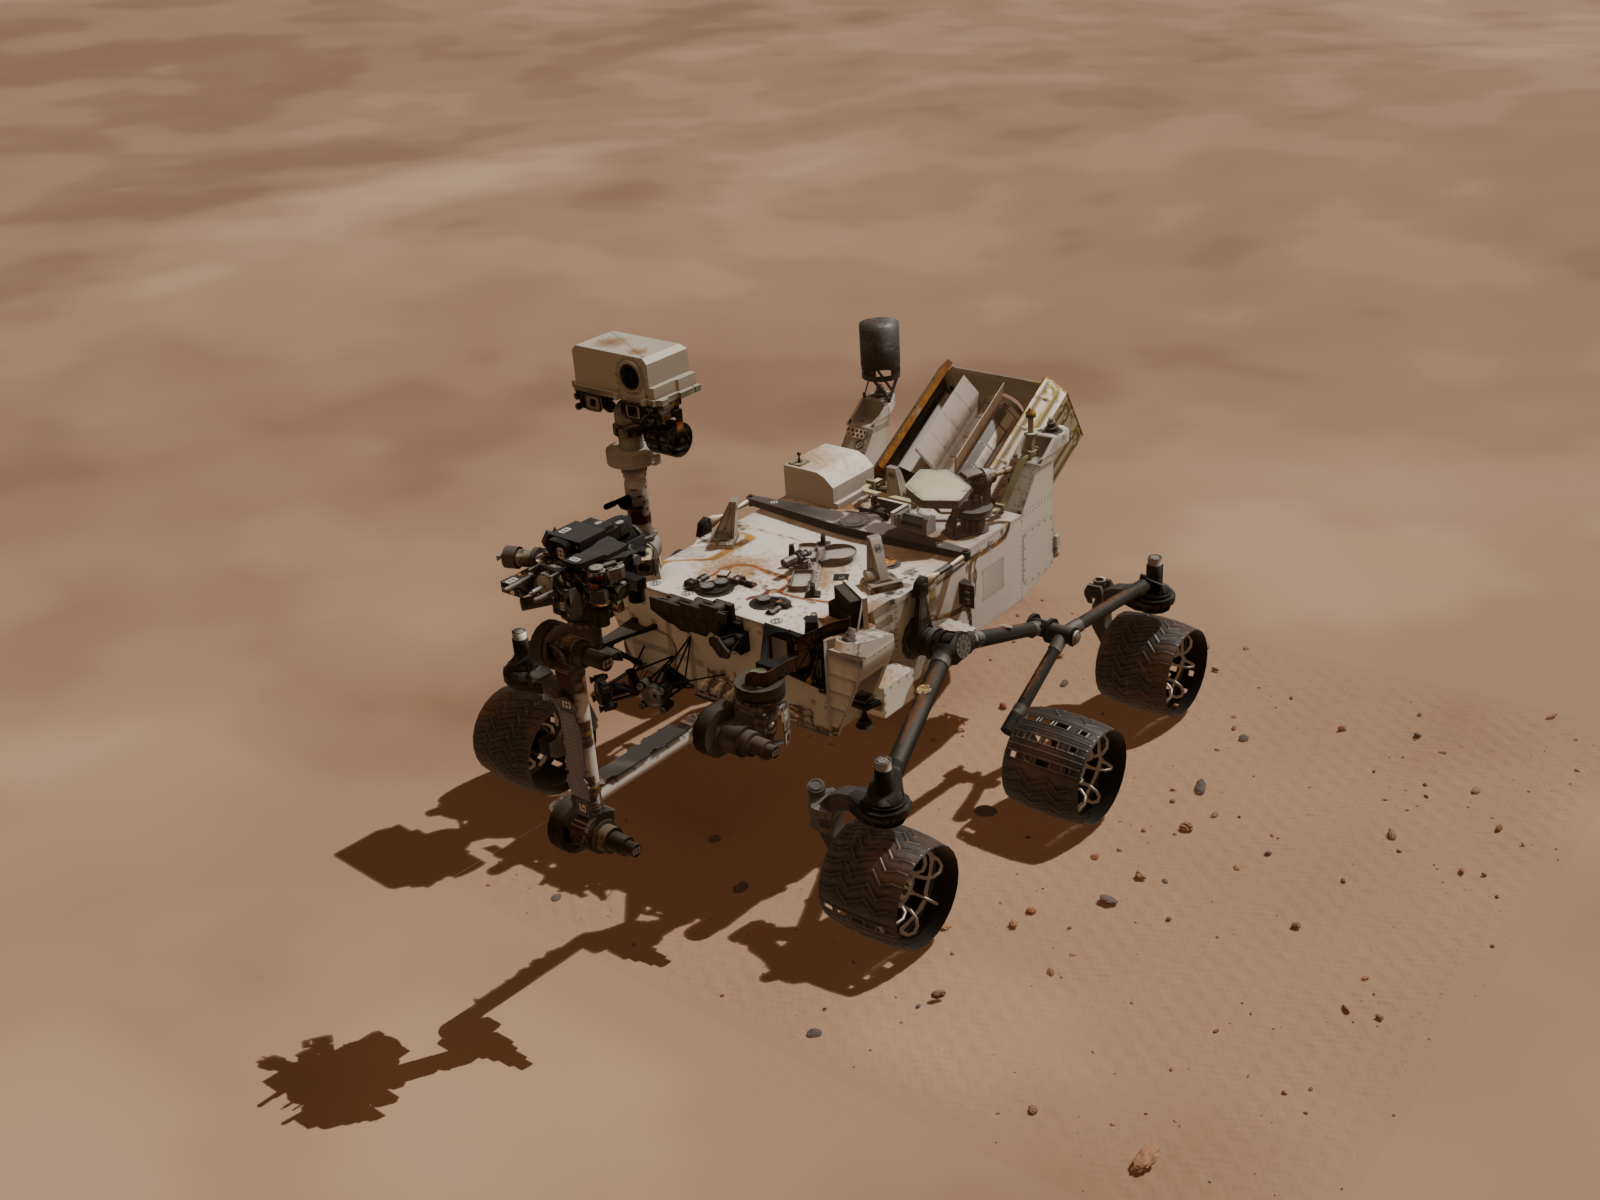
\includegraphics[width=0.70\textwidth]{Images/rover_terrain_overview_v2.png}
    \caption{Overview of the Blender scene, showing the Curiosity rover
    asset and the surrounding terrain used for synthetic image generation.}
    \label{fig:rover-terrain-scene}
\end{figure}

\section{Synthetic Damage Generation}
\label{sec:synthetic-damage-generation}
Damage generation focused on a single anomaly class: through-holes in the wheel surface, with each anomalous image containing one injected hole on the designated target wheel. Hole contours were generated procedurally using three profile families: jagged slits, branched tears, and peeled-window profiles. Variations in contour irregularity, orientation, and dimensions provided different realizations within each family. Three size-based severity levels, denoted small, medium, and large, with their length sampled within 2.7-4.1\,cm, 4.4-6.8\,cm, and 7.3-11.6\,cm, respectively. These categories describe the generated geometry rather than a mechanical assessment of wheel health. Figure~\ref{fig:damage-severity} shows an example of each level.

\begin{figure}[ht!]
    \centering
    \begin{minipage}[b]{0.32\textwidth}
        \centering
        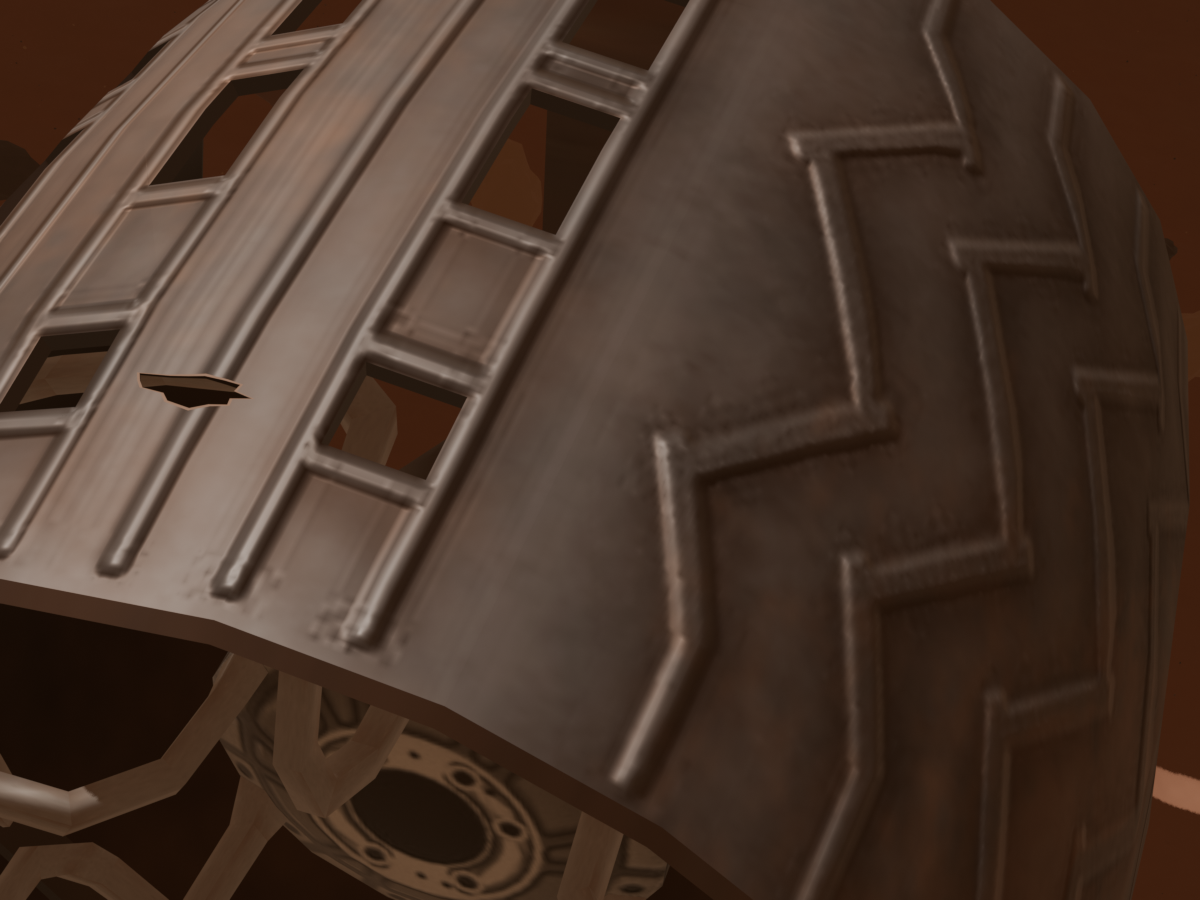
\includegraphics[width=\linewidth]{Images/hole_severity_small.png}
        \par\smallskip
        {\small (a) Small}
    \end{minipage}
    \hfill
    \begin{minipage}[b]{0.32\textwidth}
        \centering
        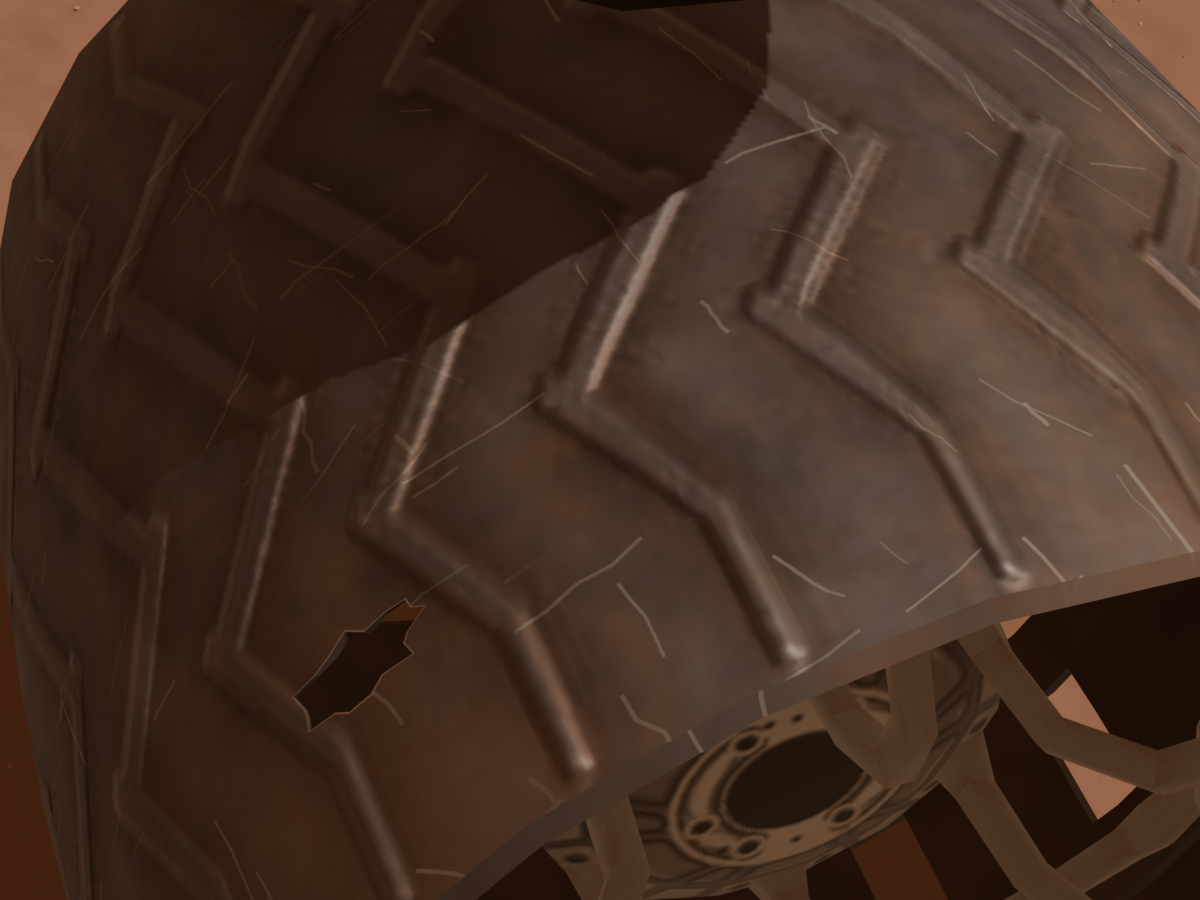
\includegraphics[width=\linewidth]{Images/hole_severity_medium.png}
        \par\smallskip
        {\small (b) Medium}
    \end{minipage}
    \hfill
    \begin{minipage}[b]{0.32\textwidth}
        \centering
        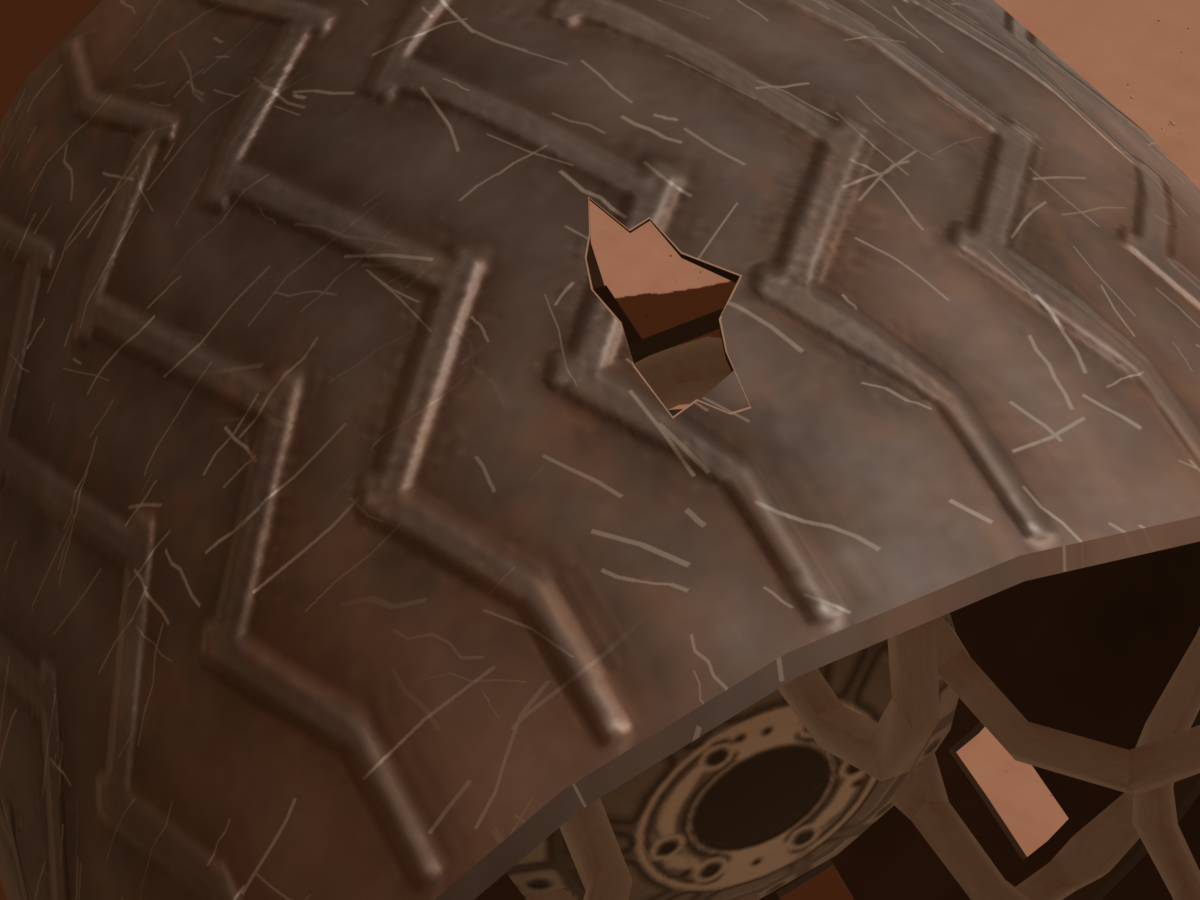
\includegraphics[width=\linewidth]{Images/hole_severity_large.png}
        \par\smallskip
        {\small (c) Large}
    \end{minipage}
    \caption{Examples of synthetic wheel damage at the three severity
    levels. The categories refer to the dimensions of the generated hole.}
    \label{fig:damage-severity}
\end{figure}

Each hole forms an opening through the wheel surface, allowing the
terrain or other rover components behind it to be seen, depending on
the viewpoint. Its appearance therefore also depends on the surrounding
scene. The hole position varied across the tread and outer shoulder. Placement
and wheel orientation were constrained so that the complete opening
remained inside the image and was not hidden by the terrain or other
rover components. For each damaged image, a corresponding binary mask
was generated automatically, providing pixel-level annotations without
manual labeling.

\section{Domain Randomization}
\label{sec:domain-randomization}

Domain randomization varies simulation conditions to expose models to a
larger range of visual appearances \cite{tobin2017domain}. In this work,
variations were introduced during rendering to diversify normal wheel
appearance and the context in which damage was observed, with the aim
of reducing reliance on specific visual cues and helping the models
distinguish actual damage from changes in appearance.

\paragraph{Lighting and dust appearance.}
Two rendering presets represented clear and dusty conditions
(Figure~\ref{fig:dr-lighting}). Alongside changes in illumination, the
dusty preset introduced deposited surface dust and a mild adjustment
to the camera response. Solar direction, direct and ambient illumination,
and exposure were also perturbed within bounded ranges. These variations
change shadows, highlights, and local contrast, requiring the detector
to distinguish an opening in the wheel from appearance changes that
can occur without damage.

\begin{figure}[htbp]
    \centering
    \begin{minipage}[b]{0.48\textwidth}
        \centering
        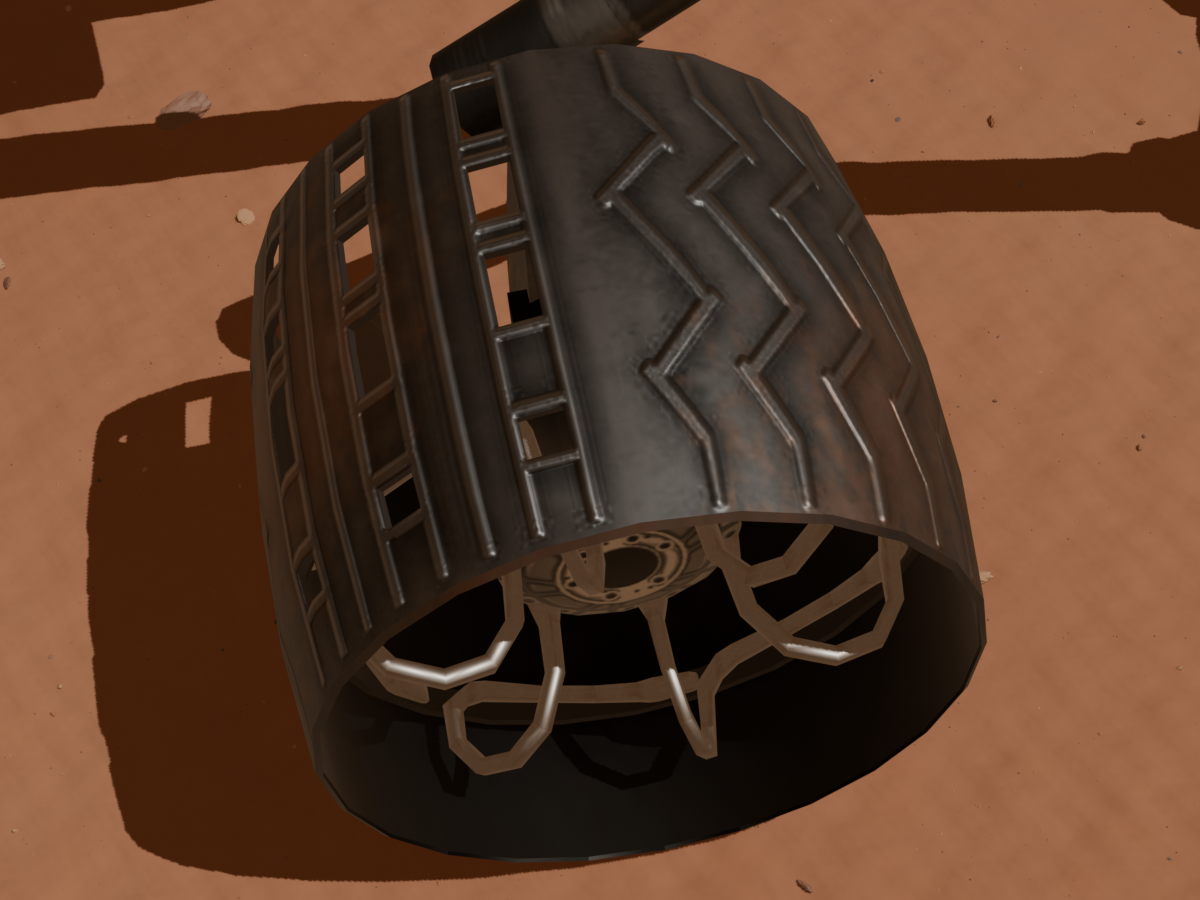
\includegraphics[width=\linewidth]{Images/dr_lighting_clear.png}
        \par\smallskip
        {\small (a) Clear preset}
    \end{minipage}
    \hfill
    \begin{minipage}[b]{0.48\textwidth}
        \centering
        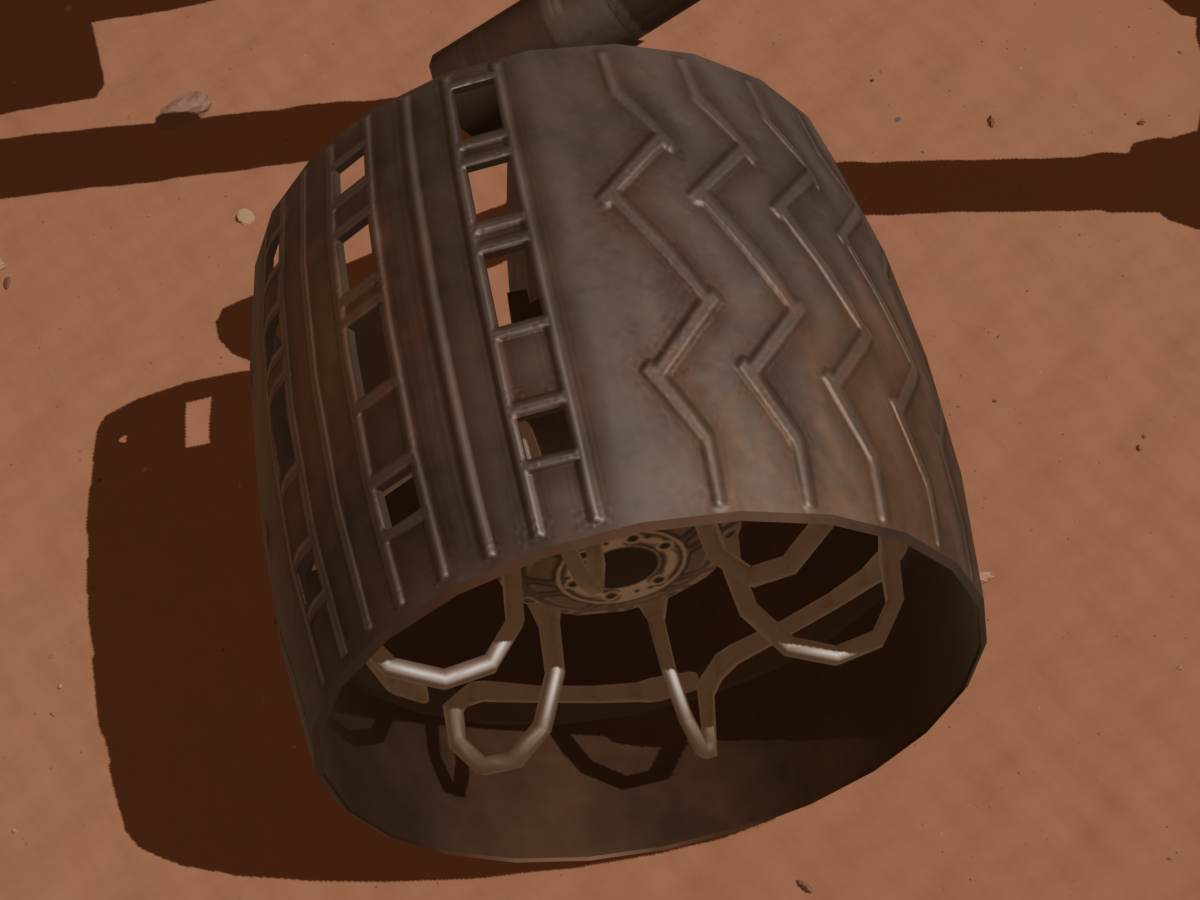
\includegraphics[width=\linewidth]{Images/dr_baseline.png}
        \par\smallskip
        {\small (b) Dusty preset}
    \end{minipage}
    \caption{Clear and dusty rendering presets applied to the same
    normal wheel, with identical camera pose and wheel orientation.
    The dusty preset also changes deposited dust and camera response,
    so the comparison does not isolate illumination alone.}
    \label{fig:dr-lighting}
\end{figure}

\paragraph{Normal surface variation.}
Three surface conditions were considered: no wear, light
wear, and evident wear (Figure~\ref{fig:dr-surface}). Additional scratches
changed the surface appearance without creating holes or altering the
wheel silhouette. Surface wear did not determine the anomaly label:
a sample was anomalous only when a hole was introduced, and scratches
were excluded from the anomaly mask. Including these patterns among
normal appearances was intended to discourage false alarms caused by
high-contrast marks or local texture changes, simulating real operational wear.

\begin{figure}[htbp]
    \centering
    \begin{minipage}[b]{0.32\textwidth}
        \centering
        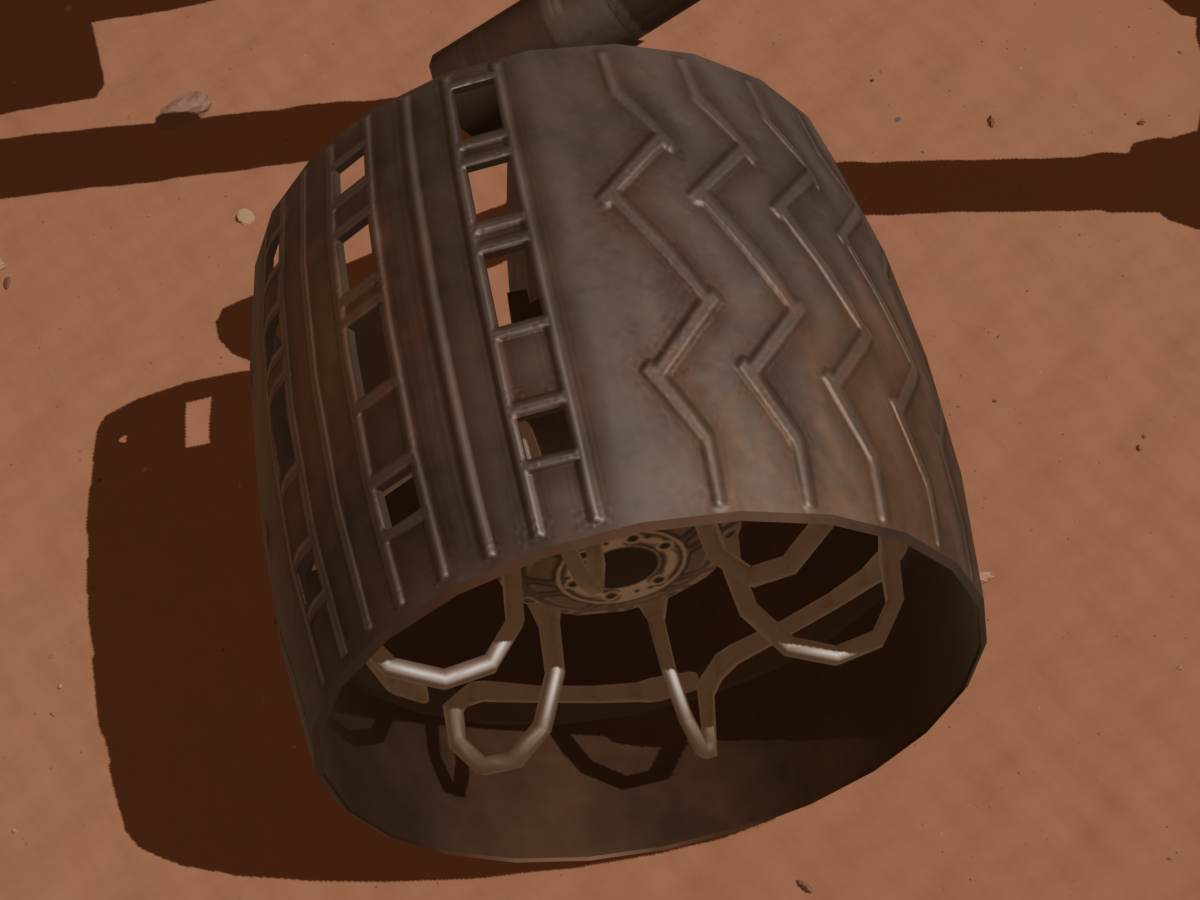
\includegraphics[width=\linewidth]{Images/dr_baseline.png}
        \par\smallskip
        {\small (a) No additional wear}
    \end{minipage}
    \hfill
    \begin{minipage}[b]{0.32\textwidth}
        \centering
        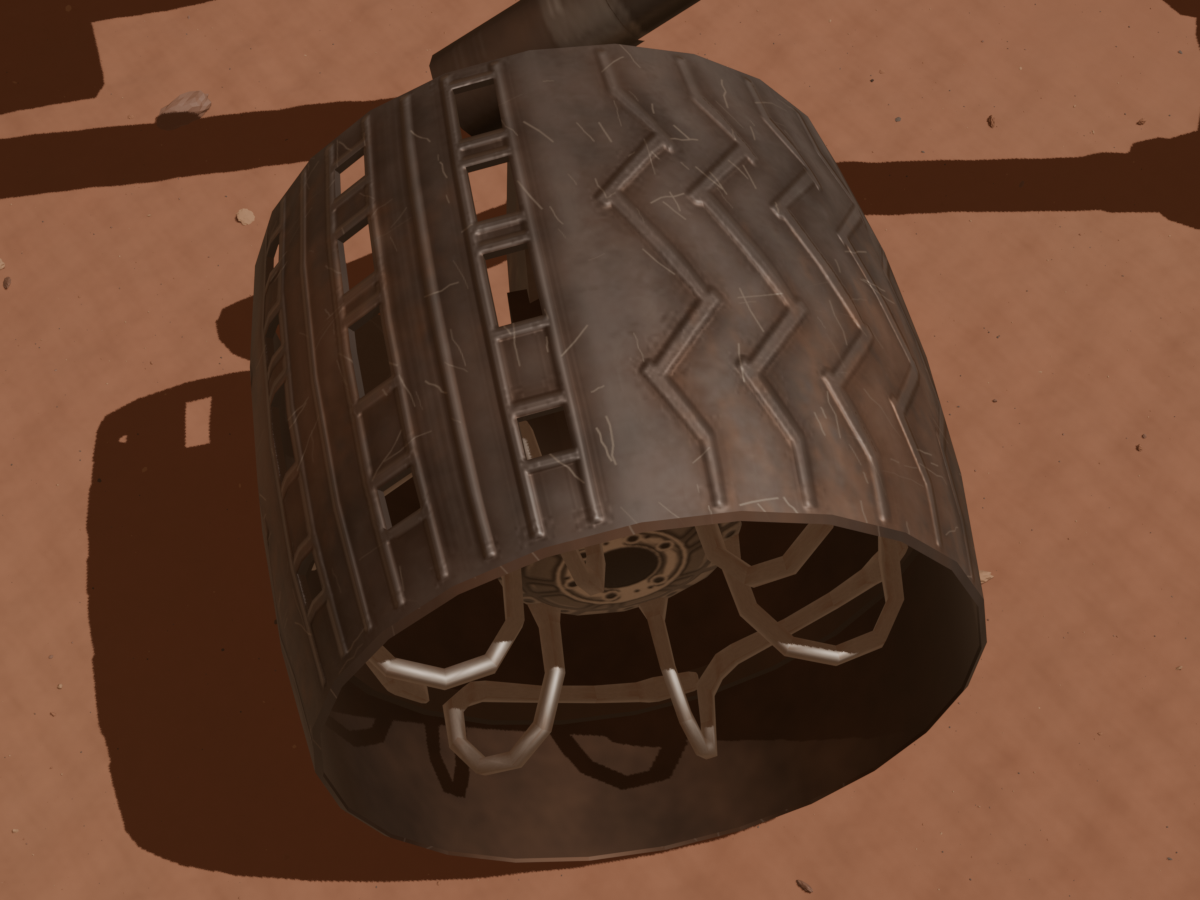
\includegraphics[width=\linewidth]{Images/dr_wear_light.png}
        \par\smallskip
        {\small (b) Light wear}
    \end{minipage}
    \hfill
    \begin{minipage}[b]{0.32\textwidth}
        \centering
        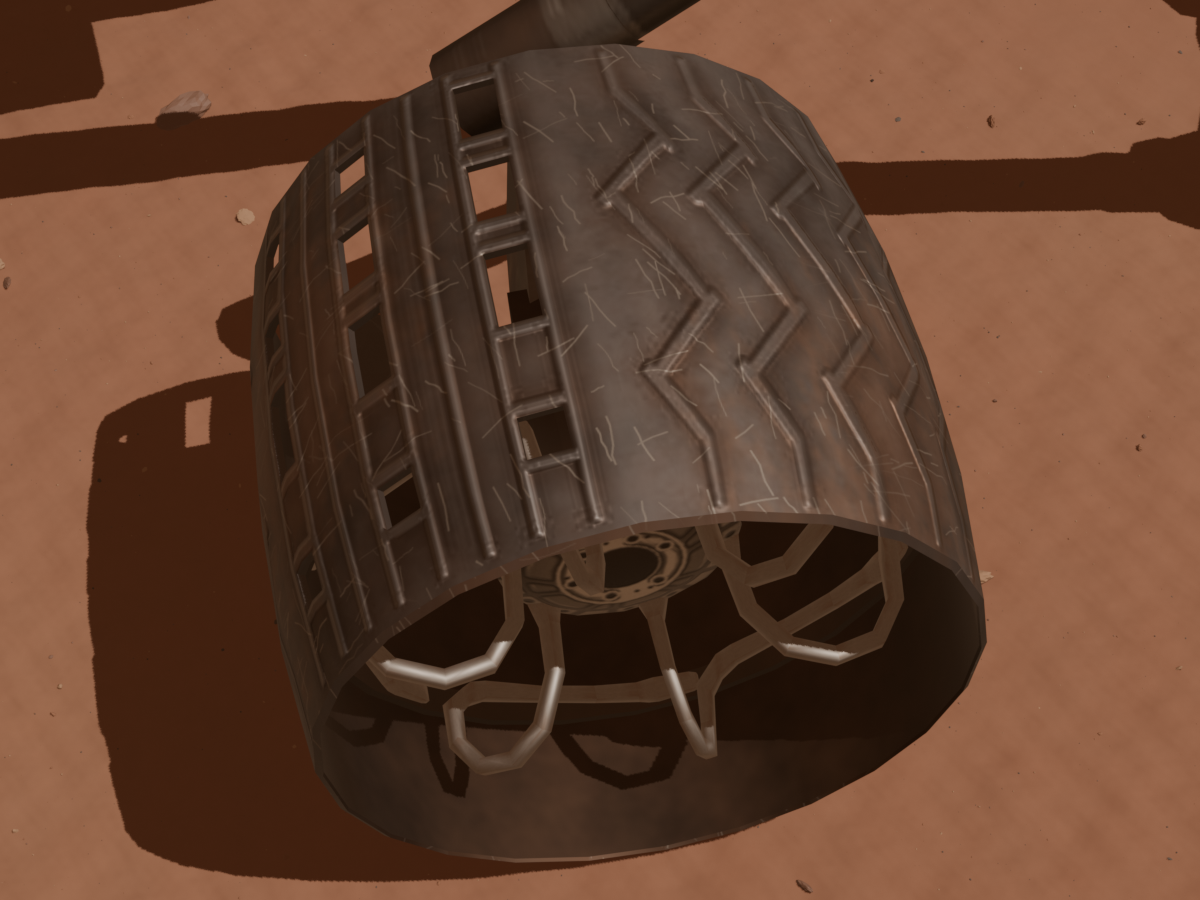
\includegraphics[width=\linewidth]{Images/dr_wear_evident.png}
        \par\smallskip
        {\small (c) Evident wear}
    \end{minipage}
    \caption{Normal surface conditions under identical lighting,
    camera pose, and wheel orientation. All three examples contain
    no injected hole and belong to the normal class.}
    \label{fig:dr-surface}
\end{figure}

\paragraph{Wheel selection and rotation.}
The target wheel was varied across all six rover wheels, introducing
different surrounding suspension and chassis structures. For standalone
normal samples, a shared rotation was applied to all six wheels using
eight phases separated by $45^\circ$. Rotation changes the visible
arrangement of tread features and surface marks, reducing dependence
on a fixed angular configuration. For damaged samples, wheel orientation
was constrained by the visibility requirements described in
Section~\ref{sec:synthetic-damage-generation}.

\paragraph{Procedural ground detail.}
The local terrain incorporated procedurally generated relief, grains,
rock fragments, and fine surface texture. These features introduce
background clutter and cast shadows near the wheel, which must be
distinguished from the target damage. The generated terrain realization
was kept throughout dataset rendering rather than regenerated for
each sample, for efficiency purposes. Its projected appearance nevertheless varied with camera pose and illumination.

\paragraph{Camera poses.}
Four wheel-centric camera configurations were used:
an overhead view (A), leading and trailing three-quarter views
(C1 and C2), and an upper detail view (D), as shown in
Figure~\ref{fig:dr-camera}. The first three configurations included
the complete wheel, whereas D intentionally captured a closer,
partial view. Small perturbations in camera position, viewing
direction, and focal length provided variation within each configuration.
Changing viewpoint modifies perspective, the visible wheel surface,
and the apparent size of a hole. Whole-wheel views retain more context
but represent small defects with fewer pixels, while the detail view magnifies local features. The different camera configurations were also included to compare detection and localization performance across viewpoints and identify the pose best suited to wheel-damage inspection.

\begin{figure}[htbp]
    \centering
    \begin{minipage}[b]{0.48\textwidth}
        \centering
        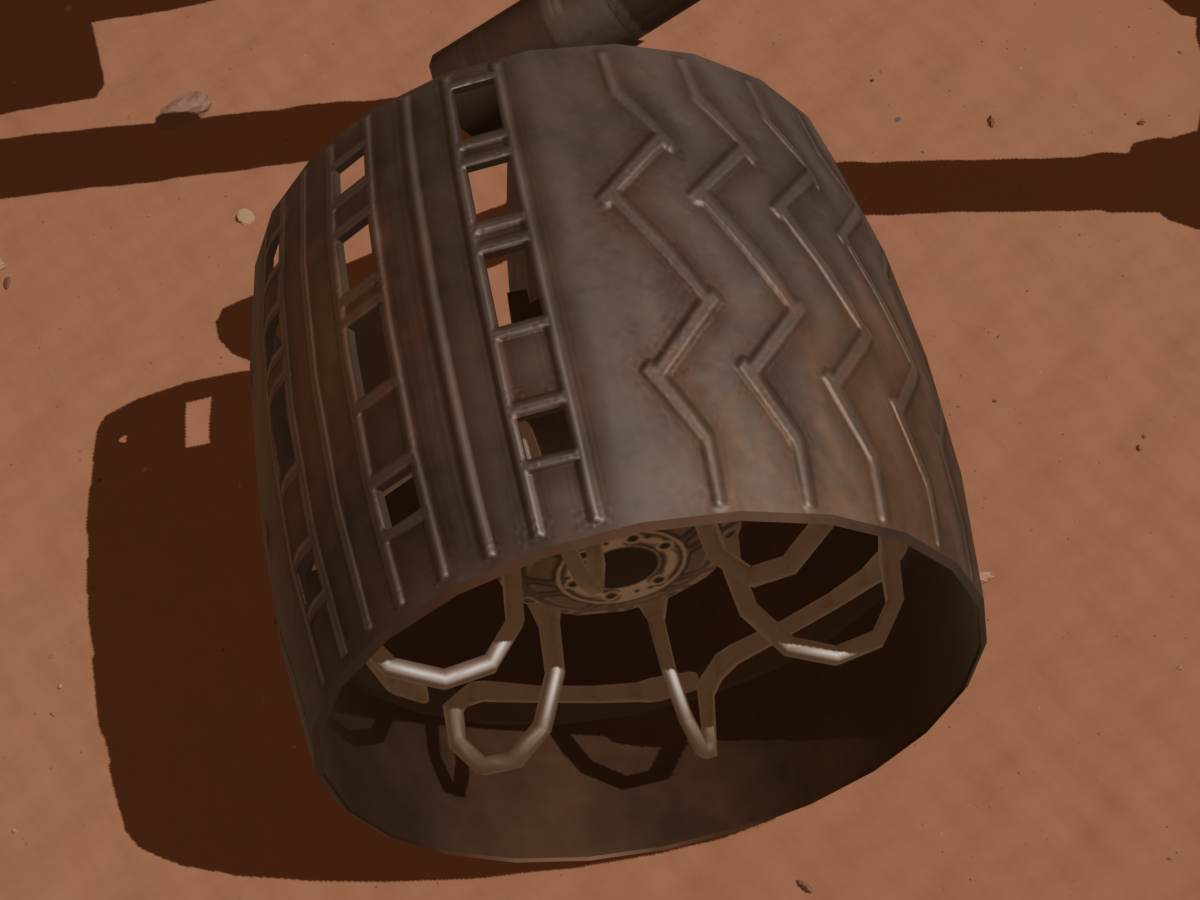
\includegraphics[width=\linewidth]{Images/dr_baseline.png}
        \par\smallskip
        {\small (a) A -- Overhead}
    \end{minipage}
    \hfill
    \begin{minipage}[b]{0.48\textwidth}
        \centering
        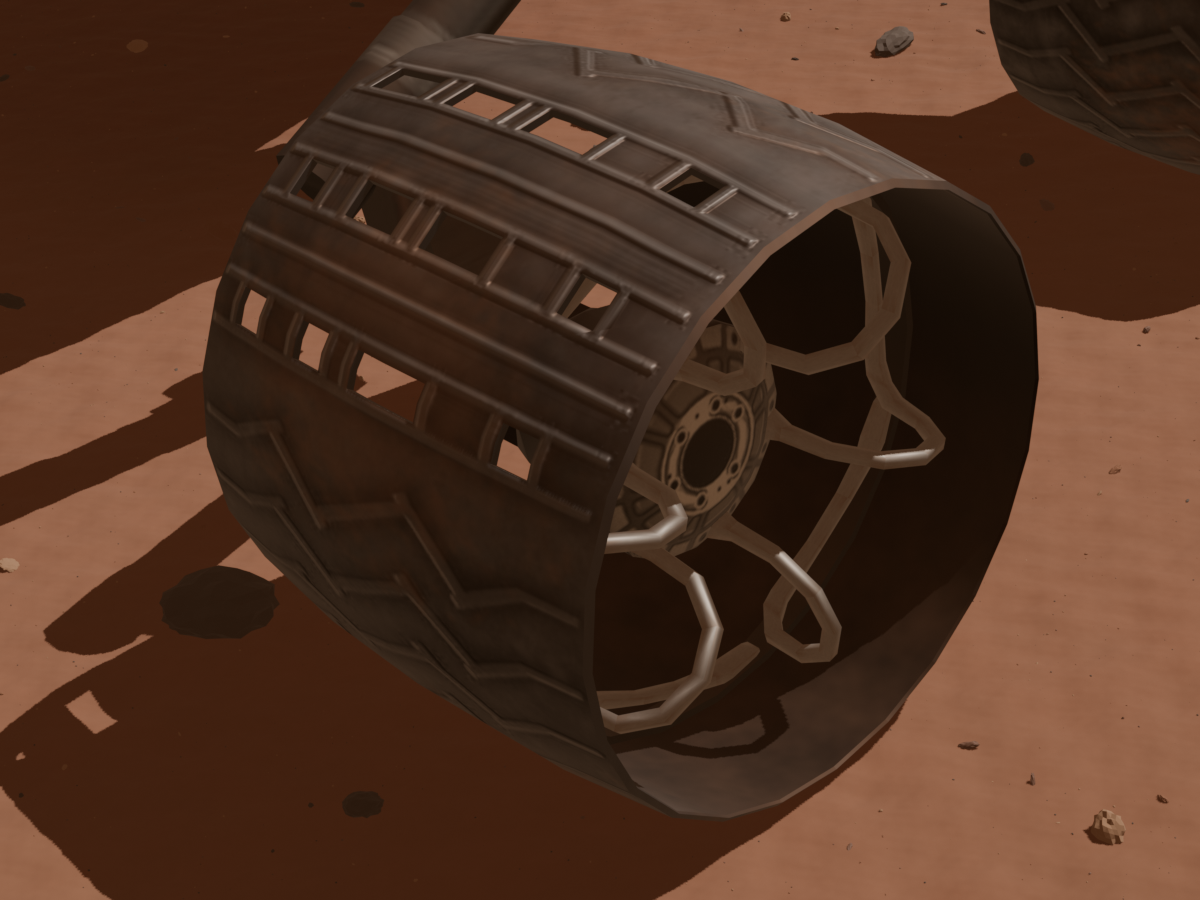
\includegraphics[width=\linewidth]{Images/dr_pose_leading.png}
        \par\smallskip
        {\small (b) C1 -- Leading three-quarter}
    \end{minipage}

    \par\medskip

    \begin{minipage}[b]{0.48\textwidth}
        \centering
        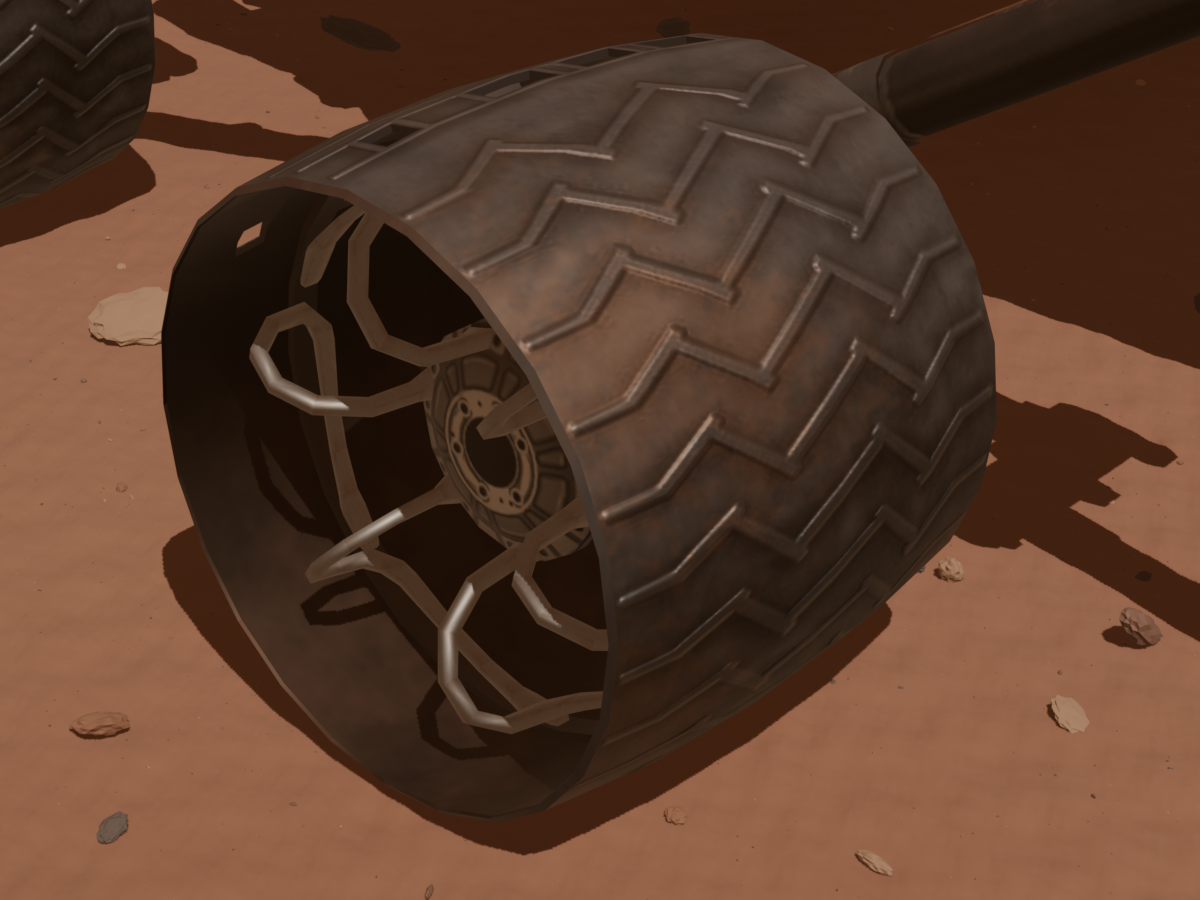
\includegraphics[width=\linewidth]{Images/dr_pose_trailing.png}
        \par\smallskip
        {\small (c) C2 -- Trailing three-quarter}
    \end{minipage}
    \hfill
    \begin{minipage}[b]{0.48\textwidth}
        \centering
        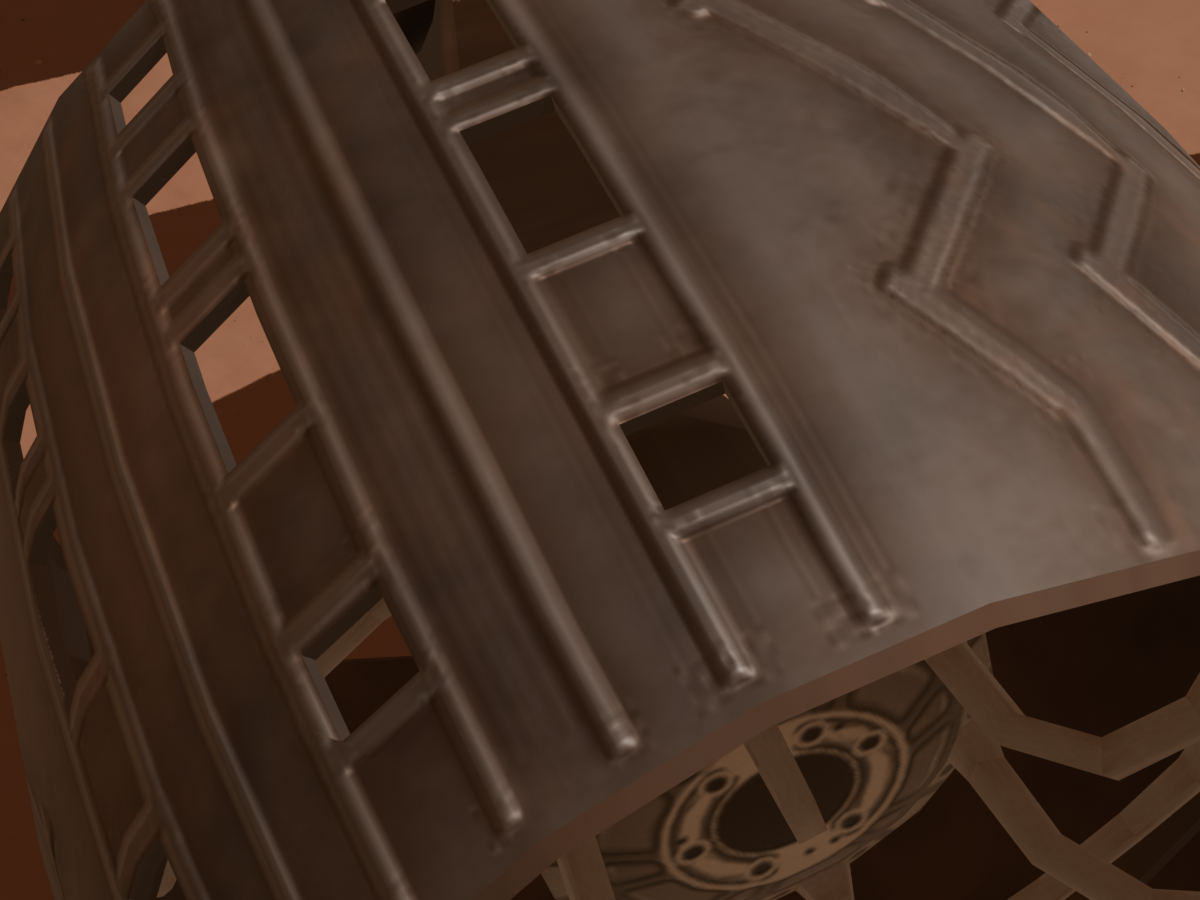
\includegraphics[width=\linewidth]{Images/dr_pose_detail.png}
        \par\smallskip
        {\small (d) D -- Upper detail}
    \end{minipage}
    \caption{The four camera configurations shown for the same
    normal wheel under the dusty preset, without additional wear.
    Wheel orientation is unchanged across views.}
    \label{fig:dr-camera}
\end{figure}

Within each clean/hole pair, lighting, surface wear, camera settings,
and wheel orientation were kept identical. Only the injected hole
distinguished the two scene states, avoiding appearance differences
that could otherwise provide unintended label cues within a pair.

\section{Quality Assurance}
\label{sec:synthetic-quality-assurance}

Quality assurance combined automated checks with visual inspection of selected renders. Geometric and annotation constraints determined sample acceptance, while contrast diagnostics identified potentially challenging examples without automatically excluding them.
The target wheel was checked for appropriate framing and unwanted occlusions. Full-wheel views required the wheel to remain within the image, whereas the partial framing of pose D was intentional and therefore admissible. For anomalous samples, the opening and its complete boundary had to remain visible. Additional checks verified wheel-ground contact and ensured that the ground region covered by the camera remained inside the detailed terrain patch, avoiding exposed patch boundaries or unsupported wheel placement.

Damage masks were required to be spatially consistent with the target-wheel region, and free of random connected components, while severity-dependent thresholds prevented annotations from becoming excessively small. Matched normal and anomalous images were compared to assess the appearance change produced by the anomalous detail and low contrast cases were kept and flagged, provided that the remaining acceptance checks were satisfied.

\section{Final Dataset Composition}
\label{sec:final-synthetic-dataset}

The final dataset contains 10,000 RGB images, comprising 7,500 normal samples and 1,250 matched normal-anomalous pairs. This results in 8,750 normal images and 1,250 anomalous images, each containing one injected hole. Every image is associated with a target-wheel mask, while anomalous images additionally include a binary damage mask.

\paragraph{Dataset splits.}
The training set contains only normal images, allowing the anomaly-detection models to learn wheel appearance without exposure to injected defects. Validation and test sets include both conditions, as summarized in Table~\ref{tab:synthetic-dataset-splits}. Validation contains 500 standalone normal images and 250 pairs, whereas the test set consists of 1,000 pairs. Split assignments were established before rendering, and each pair was treated as an indivisible unit, meaning that an anomalous image and its normal counterpart could not be assigned to different subsets.

\begin{table}[ht!]
\centering
\begin{tabular}{@{}l c c c@{}}
\toprule
\textbf{Split} & \textbf{Normal} & \textbf{Anomalous} & \textbf{Total} \\
\midrule
\midrule
Training   & 7,000 & 0     & 7,000  \\
Validation & 750   & 250   & 1,000  \\
Test       & 1,000 & 1,000 & 2,000  \\
\midrule
Total      & 8,750 & 1,250 & 10,000 \\
\bottomrule
\end{tabular}
\vspace{5mm}
\caption{Composition of the synthetic dataset across training, validation, and test splits.}
\label{tab:synthetic-dataset-splits}
\end{table}

\paragraph{Category distributions.}
The main category distributions are reported in Table~\ref{tab:synthetic-category-distributions}. The six rover wheels are represented approximately uniformly, with 1,666--1,667 images per wheel. Defect severity and placement distributions refer only to anomalous images; large defects are restricted to the tread.

\begin{table}[ht!]
\centering
\begin{tabular}{@{}l l c@{}}
\toprule
\textbf{Factor} & \textbf{Categories} & \textbf{Share (\%)} \\
\midrule
\midrule
Camera pose     & A / C1 / C2 / D           & 40 / 27.5 / 27.5 / 5 \\
Lighting        & Dusty / clear             & 75 / 25              \\
Surface wear    & Current / light / evident & 20 / 45 / 35         \\
Defect severity & Small / medium / large    & 50 / 40 / 10         \\
Defect location & Tread / outer shoulder    & 80 / 20              \\
\bottomrule
\end{tabular}
\vspace{5mm}
\caption{Main category distributions in the final dataset. Camera pose, lighting, and surface wear percentages refer to all 10,000 images; defect severity and location percentages refer to the 1,250 anomalous images.}
\label{tab:synthetic-category-distributions}
\end{table}

\paragraph{Rendering procedure.}
Images were generated through an automated batch pipeline in Blender 5.2 using Eevee, at a resolution of $1200 \times 900$ pixels with 64 rendering samples, and saved as 8-bit RGB PNG files. For each sample, the prepared scene was restored to its reference state before applying the parameters specified by the generation plan. Standalone normal samples required one render, whereas paired samples required a normal and an anomalous render with matching camera, illumination, surface appearance, and wheel configuration. Annotation information was obtained alongside the RGB renders, without separate mask-only renders; the normal target-wheel mask was retained for both members of each pair.